\documentclass[bachelor, och, referat]{../shiza}
% параметр - тип обучения - одно из значений:
%    spec     - специальность
%    bachelor - бакалавриат (по умолчанию)
%    master   - магистратура
% параметр - форма обучения - одно из значений:
%    och   - очное (по умолчанию)
%    zaoch - заочное
% параметр - тип работы - одно из значений:
%    referat    - реферат
%    coursework - курсовая работа (по умолчанию)
%    diploma    - дипломная работа
%    pract      - отчет по практике
% параметр - включение шрифта
%    times    - включение шрифта Times New Roman (если установлен)
%               по умолчанию выключен
\usepackage{subfigure}
\usepackage{tikz,pgfplots}
\pgfplotsset{compat=1.5}
\usepackage{float}

%\usepackage{titlesec}
\setcounter{secnumdepth}{4}
%\titleformat{\paragraph}
%{\normalfont\normalsize}{\theparagraph}{1em}{}
%\titlespacing*{\paragraph}
%{35.5pt}{3.25ex plus 1ex minus .2ex}{1.5ex plus .2ex}

\titleformat{\paragraph}[block]
{\hspace{1.25cm}\normalfont}
{\theparagraph}{1ex}{}
\titlespacing{\paragraph}
{0cm}{2ex plus 1ex minus .2ex}{.4ex plus.2ex}

% --------------------------------------------------------------------------%


\usepackage[T2A]{fontenc}
\usepackage[utf8]{inputenc}
\usepackage{graphicx}
\graphicspath{ {./images/} }
\usepackage{tempora}

\usepackage[sort,compress]{cite}
\usepackage{amsmath}
\usepackage{amssymb}
\usepackage{amsthm}
\usepackage{fancyvrb}
\usepackage{listings}
\usepackage{listingsutf8}
\usepackage{longtable}
\usepackage{array}
\usepackage[english,russian]{babel}

\usepackage[colorlinks=false]{hyperref}
\usepackage{url}

\usepackage{underscore}
\usepackage{setspace}
\usepackage{indentfirst} 
\usepackage{mathtools}
\usepackage{amsfonts}
\usepackage{enumitem}
\usepackage{tikz}
\usepackage{minted}

\newcommand{\eqdef}{\stackrel {\rm def}{=}}
\newcommand{\specialcell}[2][c]{%
\begin{tabular}[#1]{@{}c@{}}#2\end{tabular}}

\renewcommand\theFancyVerbLine{\small\arabic{FancyVerbLine}}

\newtheorem{lem}{Лемма}

\begin{document}

% Кафедра (в родительном падеже)
\chair{теоретических основ компьютерной безопасности и криптографии}

% Тема работы
\title{Поиск аномалий во временных рядах нейросетями}

% Курс
\course{5}

% Группа
\group{531}

% Факультет (в родительном падеже) (по умолчанию "факультета КНиИТ")
\department{факультета КНиИТ}

% Специальность/направление код - наименование
%\napravlenie{09.03.04 "--- Программная инженерия}
%\napravlenie{010500 "--- Математическое обеспечение и администрирование информационных систем}
%\napravlenie{230100 "--- Информатика и вычислительная техника}
%\napravlenie{231000 "--- Программная инженерия}
\napravlenie{100501 "--- Компьютерная безопасность}

% Для студентки. Для работы студента следующая команда не нужна.
% \studenttitle{Студентки}

% Фамилия, имя, отчество в родительном падеже
\author{Улитина Ивана Владимировича}

%Научный руководитель (для реферата преподаватель проверяющий работу)
\satitle{доцент} %должность, степень, звание
\saname{И. И. Слеповичев}

% Год выполнения отчета
\date{2024}

\maketitle

%-------------------------------------------------------------------------------------------

\tableofcontents

\intro

    \textbf{Временным рядом} называют последовательность значений, упорядоченных
    по времени, в которое то или иное значение было получено/зафиксировано. В
    качестве примеров временного ряда можно выделить:

    \begin{enumerate}
        \item курсы валют/акций (стоимость валюты/акции в конкретный момент
        времени);
        \item значение прогноза погоды, параметры работы двигателя (изменяющееся
        с течением времени значение некоторой физической величины);
        \item электрокардиограмма (биологический параметр человека);
        \item передаваемый объём сетевого трафика;
    \end{enumerate}

    Временной ряд обладает типовыми характеристиками (иногда называемые
    \textbf{компонентами}), которые точно описывают характер временного ряда и в
    виде совокупности которых временной ряд можно представить:
    
    \begin{enumerate}
        \item тренд (долгосрочное увеличение или уменьшение значений ряда);
        \item сезонность, сезонная вариация (краткосрочное регулярно
        повторяющееся колебание значений временного ряда вокруг тренда);
        \item цикл, циклические колебания (характерные изменения ряда, связанные
        с повторяющимися глобальными причинами "--- цикл деловой активности или
        экономический цикл, состоящий из экономического подъема, спада,
        депрессии и оживления);
        \item остаточная вариация, которая может быть двух видов:
            \begin{itemize}
                \item аномальная вариация — неестественно большое отклонение
                временного ряда, которое оказывает воздействие на единичное
                наблюдение;
                \item случайная вариация — малое отклонение, которое невозможно
                предвидеть.
            \end{itemize}
    \end{enumerate}


    Вследствие развития нейросетей и искусственного интеллекта, появилась
    возможность решать задачи, связанные с временными рядами, решение которых
    могло бы быть полезно для той или иной области жизнедеятельности человека.
    Особенно полезно это может быть в тех областях, где обычные статистические
    модели (обычная или интегрированная модель авторегрессии - скользящего
    среднего, векторная авторегрессия и т.д.) неприменимы или неэффективны.

    Среди задач области временных рядов можно выделить несколько наиболее
    популярных:

    \begin{enumerate}
        \item Прогнозирование следующего значения временного ряда
        \item Классификация, кластеризация, поиск паттернов временных рядов
        \item Обнаружение выбросов или аномалий во временных рядах
        \item Генерация, моделирование или выделение признаков временных рядов
        \item Модификация значений временного ряда
    \end{enumerate}

    Временные ряды могут содержать аномалии. \textbf{Аномалией} называется
    отклонение в стандартном поведении какого-то процесса, который описывается
    этим временным рядом. По сути её можно определить через аномальную вариацию,
    являющейся возможной компонентой этого временного ряда. В зависимости от
    предметной области описываемого процесса в выборке (датасете) могут быть
    аномалии разного вида. Можно выделить одни из самых распространенных видов
    аномалий:

    \begin{enumerate}
        \item точечные аномалии (наблюдается отклонение в поведении в
        отдельных точках);
        \item групповые аномалии (группа точек, которая ведет себя аномально, но
        каждая точка которой отдельно аномальной не является);
        \item контекстные аномалии, суть которых в связи аномалии с внешними
        данными, которые не присущи значениям ряда (например, отрицательная
        температура на улице летом).
    \end{enumerate}

    Настоящий реферат посвящен рассмотрению и изучению вопроса поиска аномалий
    во временных рядах с помощью нейросетей.

    Необходимость поиска аномалий может быть обусловлена тем, что обнаружение
    девиации значения процесса может способствовать улучшению решения более
    общей задачи, связанной с временным рядом этого процесса. Например, это
    может быть полезно при решении с помощью статистических моделей/моделей
    машинного обучения/нейросетей задачи классификации отрезка временного ряда
    или задачи прогнозирования. Знание того факта, что конкретный отрезок
    временного ряда содержит аномалию, наличие которой может плохо сказываться
    на обучении нейросети, дает возможность устранить аномалию для получения
    более высоких итоговых значений метрик, показывающих качество работы
    нейросети.

    Можно выделить несколько методов обнаружения аномалий:

    \begin{enumerate}
        \item STL декомпозиция, или же разложение ряда на основные компоненты;
        \item Использование изолированного леса для определения аномалий;
        \item Forecasting-based подход, или подход, основанный на определении
        аномалий с помощью предсказания значений;
        \item Clustering-based подход, или подход, основанный на решении задачи
        кластеризации;
        \item Использование автокодировщиков (глубокое обучение).
    \end{enumerate}

\section{STL декомпозиция}

        STL декомпозиция, также известная как сезонно-трендовая декомпозиция,
        основанная на LOESS (locally estimated scatterplot smoothing, или же
        локально оцененное сглаживание диаграммы рассеяния) "--- метод,
        использующий для обнаружения аномалий факт того, что временной ряд можно
        разложить на его компоненты.

        Метод эффективно работает для сезонных временных рядов (обладающих ярко
        выраженным свойством сезонности), которые являются наиболее
        распространенным типом временных рядов.

        При разложении на компоненты с последующих их визуализацией, можно
        отследить наличие аномалии. Рассмотрим пример с декомпозицией временного
        ряда, определяющих данные о продажах сома за 1996–2000 гг. Декомпозицию
        можно осуществить с помощью программного кода на Python с использованием
        библиотеки \textbf{statmodels}.

        \begin{figure}[H]
            \centering
            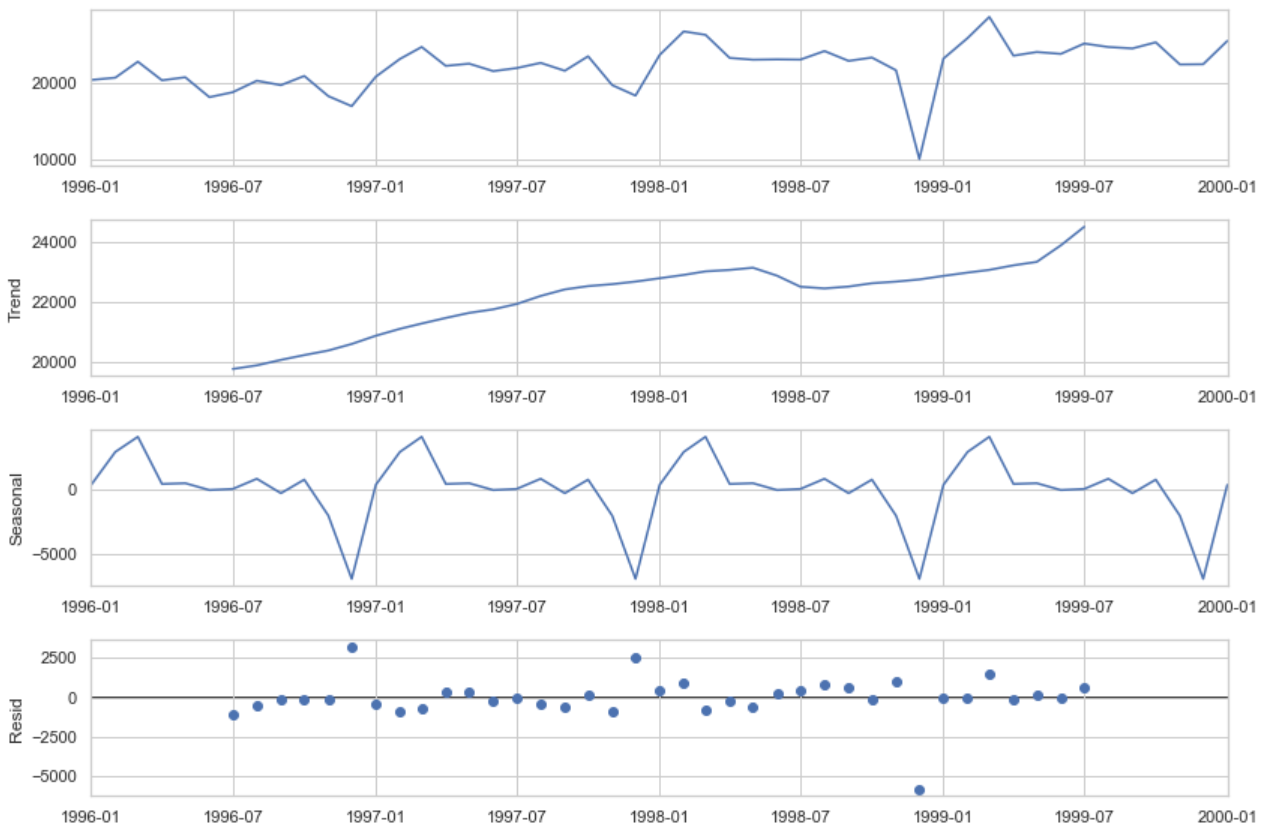
\includegraphics[width=1\textwidth]{pic/stl.png}
            \caption{Декомпозиция временного ряда (исходный ряд, тренд, сезонность, остаточная вариация)}
        \end{figure}

        На рисунке 1 на последней компоненте ряда можно наблюдать точку, сильно
        отличающуюся своим значением относительно других точек ряда. В данном
        случае совершенно необязательно использовать нейронные сети для
        определения аномалии "--- достаточно проанализировать отклонение
        последней компоненты ряда (остаточной девиации) и ввести для него
        некоторый порог, и таким образом получить простой алгоритм обнаружения
        аномалий.

        \begin{figure}[H]
            \centering
            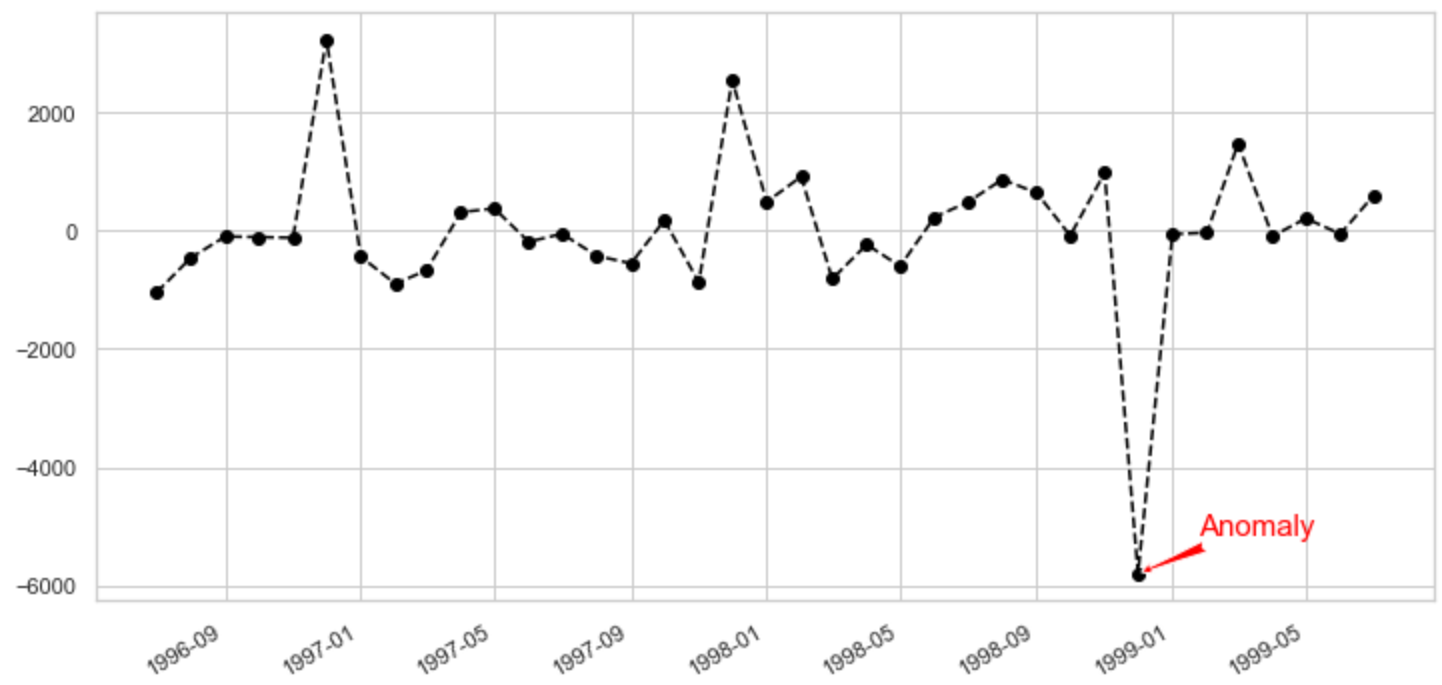
\includegraphics[width=1\textwidth]{pic/stlanom.png}
            \caption{Определение аномалии с помощью декомпозиции}
        \end{figure}

        Данный метод в контексте поиска аномалий с помощью нейросетей может быть
        полезен для предварительного преобразования временного ряда перед тем,
        чтобы применять различные нейронные сети. Например, можно использовать
        изображения отрезков временного ряда и использовать сверточные нейронные
        сети (или же их дообученные или модифицированные версии), которые будут
        работать с изображениями временного ряда.

\section{Изолированный лес}
    
        Данный метод использует популярные алгоритмы машинного обучения "---
        деревья решений и случайные леса, чтобы решать задачу выявления
        выбросов/аномалий во временных рядах.
        
        
        Можно выделить два подхода:
        \begin{enumerate}
            \item Обучение с учителем: с помощью размеченных данных (где для
            конкретных блоков временных рядов сопоставляется значение, которое
            определяет наличие аномалии в этом блоке). Однако для этого нужно
            осуществить разметку данных, которая чаще всего является трудоёмким
            процессом и занимает много времени.
            \item Обучение без учителя: можно использовать алгоритм
            изолированного леса (Isolation Forest) для предсказания наличия
            аномалии.
        \end{enumerate}
        
        Основная идея второго способа, отличающаяся от других популярных методов
        обнаружения выбросов, заключается в том, что Isolation Forest явно
        идентифицирует аномалии вместо профилирования нормальных точек данных.
        То есть Isolation Forest обнаруживает аномалии исключительно на основе
        того факта, что аномалии "--- это точки данных, которых мало и они
        отличаются от большинства. Изоляция аномалий осуществляется без
        использования каких-либо мер расстояния или энтропии (например,
        Евклидово расстояние, DTW или взаимная информация). Изолированный лес,
        как и любой метод ансамбля деревьев, основан на деревьях решений.

        Можно выделить три основных шага применения изолированного леса:

        \begin{enumerate}
            \item Для модели устанавливается значение того, какая доля выбросов
            присутствует в данных.
            \item После обучения модели совершить предсказание, тем самым
            выполнить обнаружение выбросов в данных.
            \item Визуализировать временной ряд с обнаруженными на нём
            аномалиями (например, для оценки качества определения выбросов).
        \end{enumerate}

        Листинг для выполнения всех трёх шагов выглядит примерно следующим
        образом (при этом также используются библиотеки \textbf{matplotlib,
        pandas, sklearn}):

        \begin{minted}[fontsize=\small, breaklines=true, style=bw, linenos]{Python}
            plt.rc('figure',figsize=(12,6))
            plt.rc('font',size=15)
            # визуализация исходного графика
            catfish_sales.plot()

            # определение доли выбросов
            outliers_fraction = float(.01)
            scaler = StandardScaler()
            
            # преобразование выборки для применения изолированного леса
            np_scaled = scaler.fit_transform(catfish_sales.values.reshape(-1, 1))
            data = pd.DataFrame(np_scaled)

            # обучение изолированного леса и предсказание с помощью него
            model =  IsolationForest(contamination=outliers_fraction)
            model.fit(data)
            catfish_sales['anomaly'] = model.predict(data)

            # визуализация графика с обнаруженными аномалиями
            fig, ax = plt.subplots(figsize=(10,6))
            a = catfish_sales.loc[catfish_sales['anomaly'] == -1, ['Total']] #anomaly
            ax.plot(catfish_sales.index, catfish_sales['Total'], color='black', label = 'Normal')
            ax.scatter(a.index,a['Total'], color='red', label = 'Anomaly')
            plt.legend()
            plt.show()
        \end{minted}

        С помощью программы выше можно получить результат в виде двух
        изображений на рисунке 3.

        \begin{figure}[H]
            \centering
            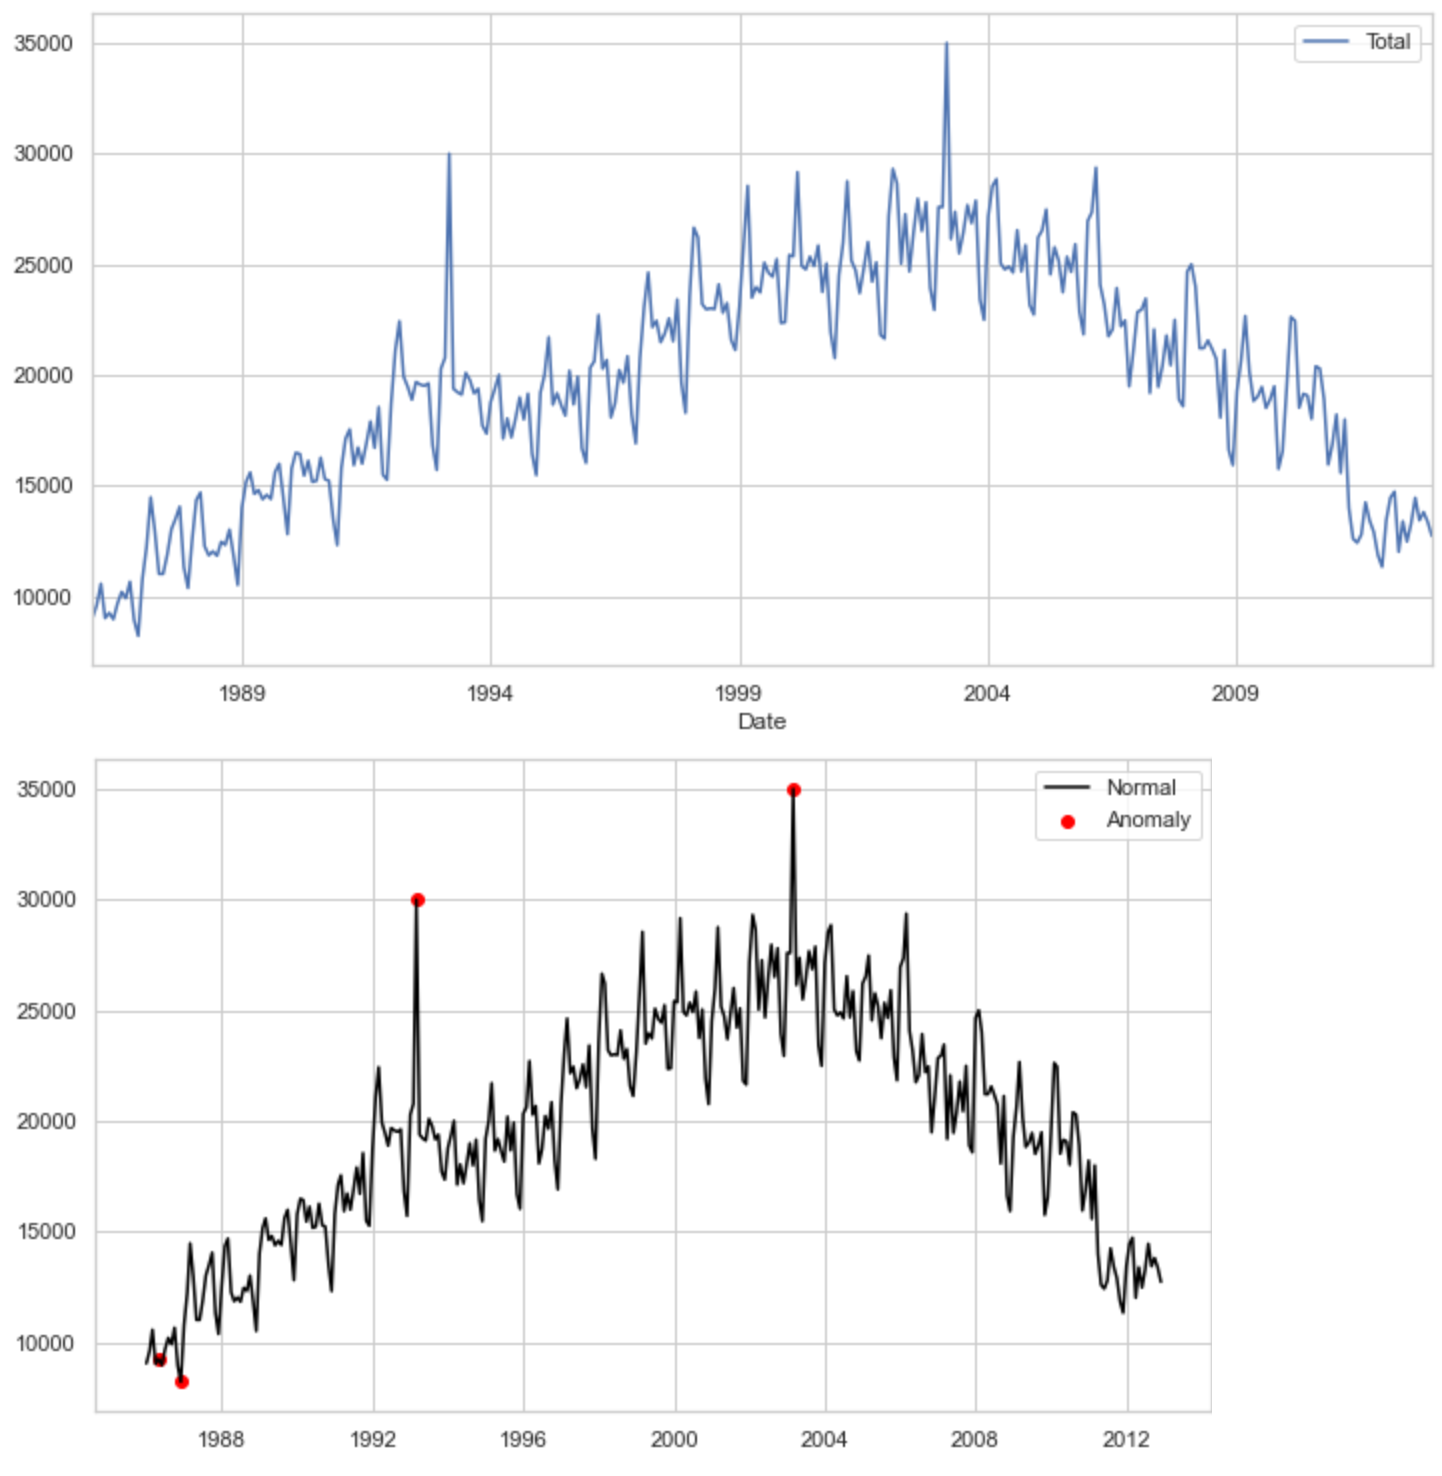
\includegraphics[width=1\textwidth]{pic/forest.png}
            \caption{Обнаружение аномалий с помощью изолированного леса}
        \end{figure}
    
        Хоть деревья решений это не нейронные сети, а методы машинного обучения,
        нельзя не сказать об их возможной эффективности решения данной задачи
        без применения методов глубокого обучения. Кроме того, не исключена
        возможность применения данных алгоритмов в качестве элементов ансамбля,
        в котором следующим элементом после изолированного леса будет
        применяться нейронная сеть.
    
\section{Forecasting-based подход}
    
        Обнаружение аномалий с помощью прогнозирования основано на подходе, при
        котором на основе нескольких точек из прошлого генерируется значение
        следующей точки с добавлением некоторой случайной величины, которая
        обычно представляет собой белый шум. Таким образом можно осуществить
        предсказание нескольких значений сигнала подряд, что будет влиять на
        горизонт дальнейшего прогноза "--- спрогнозированный далее сигнал
        становится более плавным, гладким. Следовательно, те значения временного
        ряда, которые будут значительно отличаться от спрогнозированного,
        являются выбросами.

        Сложность использования этого метода заключается в том, чтобы выбрать
        то, по каким признакам и параметрам будет осуществляться проверка на
        различия двух значений временного ряда "--- будь то значение их
        разности, или же что-то более универсальное и общее, например: 

        \begin{enumerate}
            \item общее расстояние между блоками временного ряда (например,
            Евклидово), которое определяется следующей формулой:

            $$Euc(x, y) = \bigg(\sum |(x_i - y_i)|^2 \bigg)^\frac{1}{2},$$
            
            где $x_i$ "--- $i$-е значение первого временного ряда $x$, $y_i$
            "--- $i$-е значение второго временного ряда $y$;

            \item значение взаимной информации:
    
            $$MI(x,y)=\sum_{i=1}^{|x|} \sum_{j=1}^{|y|} \frac{|x_i\cap y_j|}{N}
            \log\frac{N|x_i \cap y_j|}{|x_i||y_j|},$$

            где $x_i$ "--- $i$-е значение первого временного ряда $x$, $y_i$
            "--- $i$-е значение второго временного ряда $y$, $N = |x| + |y|$;

            \item значение динамической трансформации временной шкалы (DTW, или
            же dynamic time warping):

            $$DTW(x, y) = \min_\pi \sqrt{ \sum_{(i, j) \in \pi} d(x_i, y_j)^2
            },$$

            где $x_i$ "--- $i$-е значение первого временного ряда $x$, $y_i$
            "--- $i$-е значение второго временного ряда $y$, $\pi = [\pi_0,
            \dots , \pi_K]$ "--- это путь, который удовлетворяет следующим
            свойствам:

            \begin{itemize}
                \item это список пар индексов $\pi_k = (i_k, j_k)$ с $0 \leq i_k
                < n$ и $0 \leq j_k < m$
                \item $\pi_0 = (0, 0)$ и $\pi_K = (n - 1, m - 1)$
                \item $\forall k > 0, \pi_k = (i_k, j_k)$ относится к $\pi_{k-1}
                = (i_{k-1}, j_{k-1})$ следующим образом: $i_{k-1} \leq i_k \leq
                i_{k-1} + 1$ и $j_{k-1} \leq j_k \leq j_{k-1} + 1$.
            \end{itemize}

            Здесь путь можно рассматривать как временное выравнивание временных
            рядов, при котором евклидово расстояние между выровненными
            временными рядами минимально.


        \end{enumerate}
        
        Еще одним препятствием является то, что после дифференциации сигнала он
        должен оставаться стационарным. Это означает, что сигнал не должен
        зависеть от времени, что является существенным ограничением.

        Для применения данного метода необходимо использовать некоторую модель
        для прогнозирования значения временного ряда, будь то модель нейронной
        сети или же некоторая статистическая модель:

        \begin{enumerate}
            \item ARMA (модель авторегрессии - скользящего среднего). Модель
            ARMA обобщает две более простые модели временных рядов "--- модель
            авторегрессии (AR) и модель скользящего среднего (MA);
            \item ARIMA (модель Бокса — Дженкинса) "--- является расширением
            моделей ARMA для нестационарных временных рядов;
            \item SARIMA (модель сезонного авторегрессивного интегрированного
            скользящего среднего) "--- расширение модели ARIMA, основанной на
            концепции сезонных трендов. SARIMA вместе со своими
            предшественниками представляет группу наиболее распространенных
            математических моделей, использующихся для анализа и прогнозирования
            стационарных временных рядов в статистике;
            \item RNN (рекуррентные нейронные сети) "--- вид нейронной сети,
            который хорошо подходит для задач обработки последовательностей
            данных (которыми в том числе могут являться временные ряды);
            \item LSTM (long short-term memory) "--- рекуррентная нейронная
            сеть, направленная на решение проблемы исчезающего градиента,
            характерной для рекуррентной нейронной сети.
        \end{enumerate}

        Рассмотрим последние две более подробно.

        \subsection{RNN}

            Рекуррентная нейронная сеть или РНС (англ. Recurrent Neural Network,
            RNN) "--- это тип искусственной нейронной сети, которая обрабатывает
            последовательности данных и временные ряды. Подобно нейронным сетям
            с прямой связью (англ. Feedforward Neural Network, FNN) и CNN,
            рекуррентные нейронные сети используют обучающие данные для
            изменения своих весов. Основным отличием от других видов сетей
            является ''память'', суть которой в том, что в процессе обработки
            входной информации особым текущим слоем в RNN, используются входные
            параметры к некоторым предыдущим слоям сети (таким образом влияя на
            результат работы текущего слоя сети). В то время как традиционные
            глубокие нейронные сети предполагают, что входные и выходные данные
            слоев независимы друг от друга, выходы рекуррентных нейронных сетей
            зависят от предшествующих элементов внутри последовательности этих
            слоев. Хотя будущие преобразования также могут быть полезны для
            определения результата данной последовательности, однонаправленные
            рекуррентные нейронные сети не могут учитывать эти преобразования в
            своих прогнозах.

            Однако при использовании первых архитектур RNN возникала проблема
            потери способности связывать информацию в силу уменьшения влияния
            аргументов слоев сети на текущий обрабатываемый слой по мере
            увеличения ''расстояния'' между слоем, для которого были изначально
            предназначены аргументы, и текущим слоем. Уменьшение влияния
            выражается через проблему исчезающего градиента (англ. Vanishing
            gradient problem), которая возникает в процессе обучения ANN с
            помощью методов, основанных на градиентном спуске (англ. Gradient
            Descent) и методе обратного распространения ошибки (англ.
            Backpropagation). В этих способах обучения, на протяжении всей
            итерации обучения или эпохи, каждый из весов нейросети обновляется
            пропорционально частной производной функции ошибки от текущего веса.
            Время от времени значение градиента может становиться бесконечно
            малым, что препятствует обновлению значения веса. На практике, в
            силу отсутствия возможности сохранения качества передачи параметров
            между слоями, была представлена реализация модификации рекуррентной
            нейросети, которая способна к обучению долговременным зависимостям.
            Название такого подкласса RNN "--- сеть с долгой краткосрочной
            памятью (англ. Long Short-Term Memory, LSTM).

            \begin{figure}[H]
                \centering
                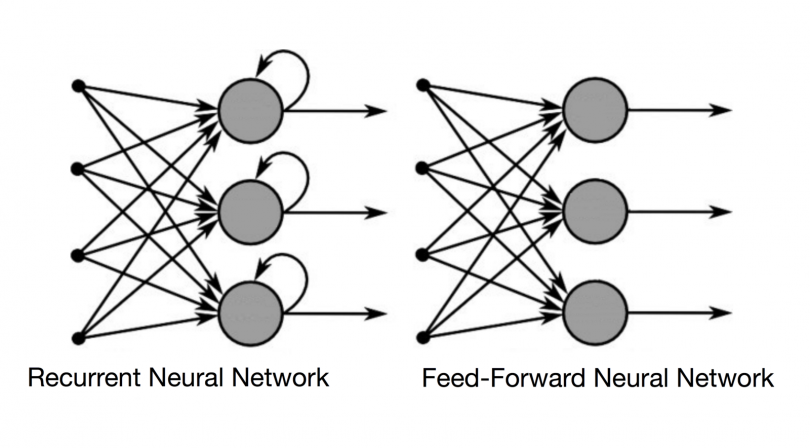
\includegraphics[width=0.8\textwidth]{pic/rnn-vs-fnn.png}
                \caption{Абстрактное сравнение архитектур FNN и RNN}
            \end{figure}

        \subsection{LSTM}

            Решение с помощью LSTM использует ''карусель с постоянными
            ошибками'' (англ. Constant Error Carousel, CEC), которые
            обеспечивают постоянный поток ошибок (необходимый для хранения
            значений ошибки для дальнейшего обучения модели) в специальных
            ячейках. Доступ к ячейкам (и их применение) осуществляется
            мультипликативными блоками ворот (англ. gate units), которые учатся
            своевременно предоставлять этот доступ. CEC являются центральной
            функцией LSTM, где осуществляется хранение краткосрочной памяти в
            течении длительных периодов времени. В ходе выполнения обработки
            соединений между другими блоками сети LSTM может также возникнуть
            конфликт обновления веса. Входные соединения некоторого нейрона $u$
            могут конфликтовать в процессе обновления веса по причине того, что
            один и тот же вес может как использоваться для хранения некоторого
            входного значения, так и не использоваться. Для взвешенных выходов
            соединений, идущих от нейрона $u$, одинаковые веса могут вернуть
            содержимое $u$ и сделать поток вывода ошибки в другие нейроны сети
            некорректным. Эту проблему решает расширение CEC входными и
            выходными блоками ворот, которые соединены с входным слоем сети и с
            другими ячейками памяти, что ведет к формированию особого блока
            LSTM, называемого блоком памяти (англ. Memory Block).

            \begin{figure}[H]
                \centering
                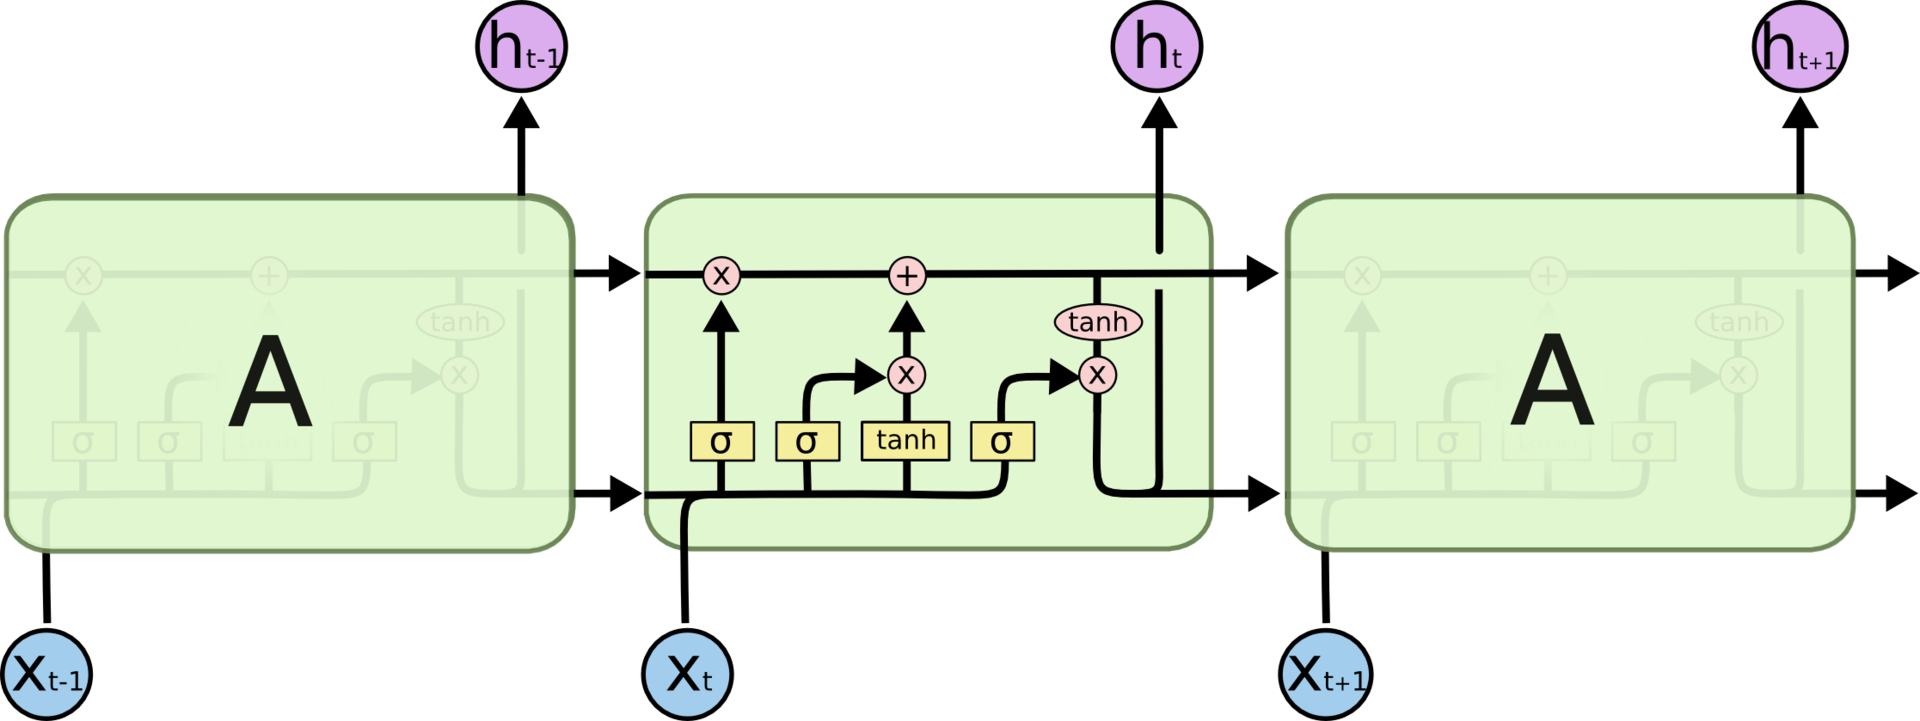
\includegraphics[width=0.8\textwidth]{pic/lstm.png}
                \caption{Схема содержимого модуля LSTM-сети}
            \end{figure}

            Таким образом, для каждого элемента входной последовательности
            каждый $t$-ый слой LSTM модели осуществляет следующие вычисления:
    
            \[i_t = \sigma(W_{ii} x_t + b_{ii} + W_{hi} h_{t - 1} + b_{hi}) ;\]
            \[f_t = \sigma(W_{if} x_t + b_{if} + W_{hf} h_{t - 1} + b_{hf}) ;\]
            \[g_t = \tanh(W_{ig} x_t + b_{ig} + W_{hg} h_{t - 1} + b_{hg}) ;\]
            \[o_t = \sigma(W_{io} x_t + b_{io} + W_{ho} h_{t - 1} + b_{ho}) ;\]
            \[c_t = f_t \odot c_{t - 1} + i_t \odot g_t ;\]
            \[h_t = o_t \odot \tanh(c_t) ,\]
    
            где $h_t, c_t, x_t$ "--- скрытое состояние слоя модели, состояние
            клетки и входной параметр в момент времени $t$ соответственно; $h_{t
            - 1}$ определяет скрытое состояние слоя в момент времени $t - 1$ или
            начальное скрытое состояние в момент времени $o$. Элементы $i_t,
            f_t, g_t, o_t$ являются входными, забывающими, клеточными и
            выходными воротами соответственно. Символ $\sigma$ определяет
            функцию сигмоиды, $\odot$ "--- поэлементное произведение, также
            называемое произведением Адамара.

\section{Clustering-based подход}
    
        Если вернуться к теме применения методов определения аномалий,
        предполагающих обучение без учителя, то следует упомянуть подход,
        связанный с кластеризацией.

        Подход подразумевает рассмотрение элементов выборки как точек в
        пространстве, которые можно определить в группы ближайших друг к другу
        точек "--- кластеров. Элементы выборки, выходящие за пределы
        определенных кластеров, потенциально могут быть помечены как аномалии.
        
        Существует несколько методов кластеризации, среди которых можно
        выделить:

        \begin{enumerate}
            \item Метод $k$-средних (англ. $k$-means) "--- итеративный алгоритм,
            основанный на минимизации суммарного квадратичного отклонения точек
            кластеров от центров этих кластеров;
            \item Распространение похожести (англ. affinity propagation) "---
            распространяет информацию о похожести между парами объектов для
            выбора типичных представителей каждого кластера;
            \item Сдвиг среднего значения (англ. mean shift) "--- выбирает
            центроиды кластеров в областях с наибольшей плотностью.
        \end{enumerate}

        Далее будет рассмотрен пример применения $k$-средних на выборке
        многомерного временного ряда. Однако, чтобы применить этот метод,
        необходимо указать количество кластеров, на которые следует делить
        элементы выборки. Для этого можно использовать метод локтя (англ. Elbow
        method). Метод локтя представляет собой график зависимости количества
        кластеров от оценки дисперсии. Чтобы реализовать это, можно использовать
        реализацию $k$-средних в \textbf{sklearn}:

        \begin{minted}[fontsize=\small, breaklines=true, style=bw, linenos]{Python}
            data = df[['price_usd', 'srch_booking_window', 'srch_saturday_night_bool']]
            n_cluster = range(1, 20)
            kmeans = [KMeans(n_clusters=i).fit(data) for i in n_cluster]
            scores = [kmeans[i].score(data) for i in range(len(kmeans))]
            fig, ax = plt.subplots(figsize=(10,6))
            ax.plot(n_cluster, scores)
            plt.xlabel('Number of Clusters')
            plt.ylabel('Score')
            plt.title('Elbow Curve')
            plt.show()
        \end{minted}

        Таким образом можно получить следующее изображение:

        \begin{figure}[H]
            \centering
            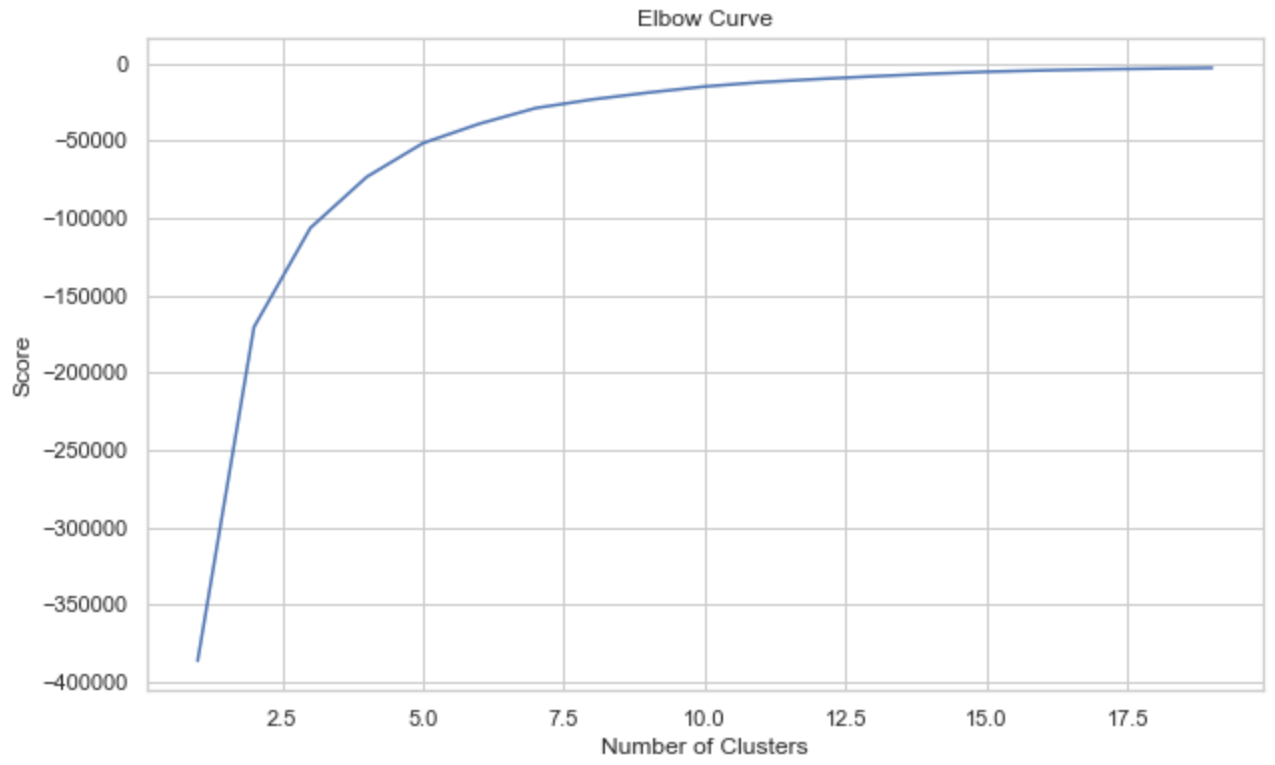
\includegraphics[width=1\textwidth]{pic/elbow.png}
            \caption{График для метода локтя}
        \end{figure}

        Из приведенного выше рисунка видно, что график выравнивается после $10$
        кластеров, а это означает, что добавление большего количества кластеров
        не способствует более эффективному разделению элементов выборки.

        Таким образом, определение аномалий можно осуществить сначала
        относительно кластеров, а затем применить полученные результаты
        относительно исходного временного ряда.

        \begin{figure}[H]
            \centering
            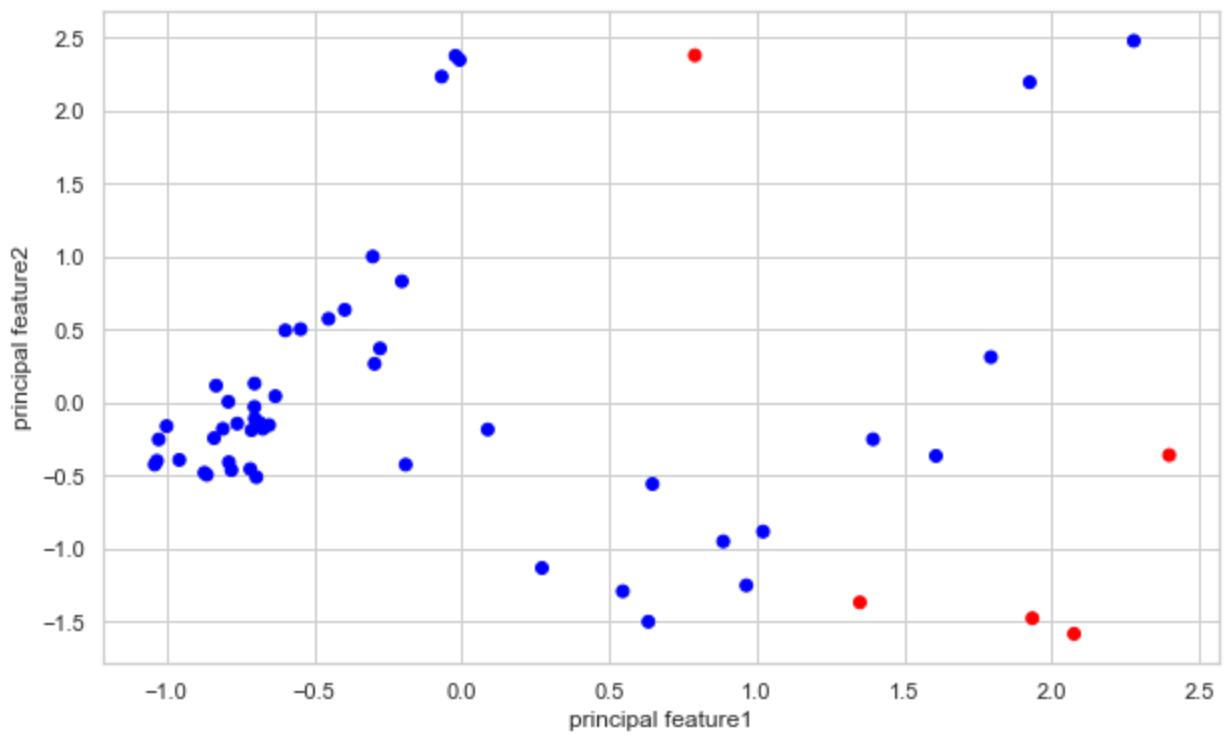
\includegraphics[width=1\textwidth]{pic/clust1.png}
            \caption{Определение аномалий относительно кластера}
        \end{figure}

        \begin{figure}[H]
            \centering
            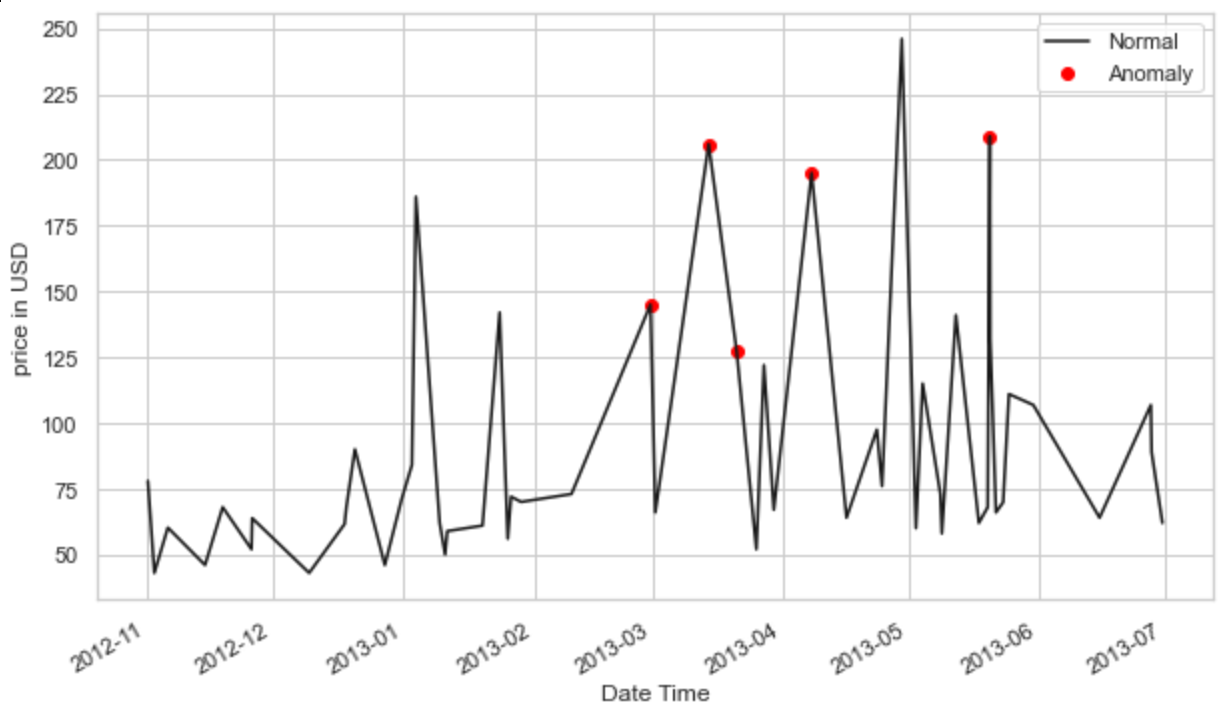
\includegraphics[width=1\textwidth]{pic/clust2.png}
            \caption{Определение тех же аномалий на исходном временном ряду}
        \end{figure}

\section{Автокодировщики}

    Автокодировщик (англ. autoencoder) "--- специальная архитектура
    искусственных нейронных сетей, позволяющая применять обучение без учителя
    при использовании метода с обратного распространения ошибки. Простейшая
    архитектура автокодировщика "--- сеть прямого распространения, без обратных
    связей, наиболее схожая с перцептроном и содержащая входной слой,
    промежуточный слой и выходной слой. В отличие от перцептрона, выходной слой
    автокодировщика должен содержать столько же нейронов, сколько и входной
    слой.

    Автокодировщик включает в себя кодировщик (который преобразует входной
    сигнал в код) и декодировщик (который восстанавливает сигнал по его коду).
    Скрытый слой автокодировщика называется bottleneck-слоем, ключевая
    особенность которого "--- наименьшая размерность из всех скрытых слоев.
    Размерность слоев автокодировщика при переборе от входного слоя к
    bottleneck-слою последовательно уменьшается, а при переборе от
    bottleneck-слоя к выходному слою последовательно увеличивается. Набор слоев
    автокодировщика от входного до bottleneck-слоя называется кодировщиком, а от
    bottleneck к выходному "--- декодировщиком.

    \begin{figure}[H]
        \centering
        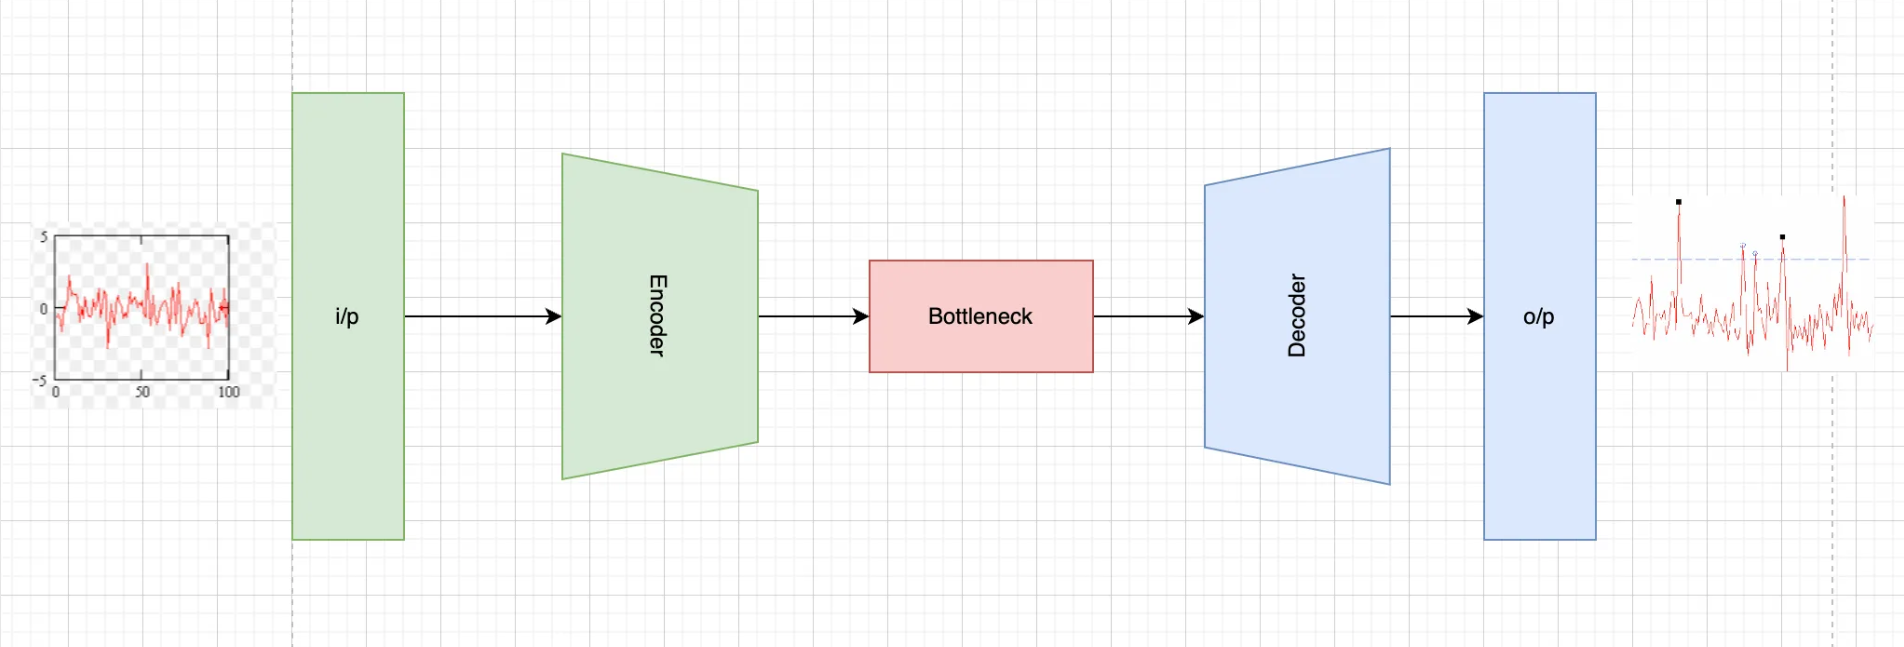
\includegraphics[width=1\textwidth]{pic/autoenc.png}
        \caption{Абстрактная схема автокодировщика}
    \end{figure}

    В данном случае применение скрытого представления данных автокодировщика
    аналогично уменьшению размерности.

    При уменьшении размерности таким образом выявляются как основные
    закономерности в данных, так и выбросы/аномалии. Многие методы, основанные
    на расстоянии (например, kNN "--- метод $k$ ближайших соседей), страдают от
    проклятия размерности при вычислении расстояния между всеми точками данных в
    полном пространстве признаков. Поэтому большую размерность может быть
    полезно уменьшать.

    Основное преимущество по сравнению с методом главных компонент (PCA) в том,
    что автокодировщик (в отличии от PCA) может осуществлять нелинейные
    преобразования с помощью нелинейной функции активации и нескольких слоев.
    Более эффективно обучать несколько слоев с помощью автокодировщика, чем
    обучать одно огромное преобразование с помощью PCA. Таким образом,
    автокодировщик особенно эффективен при сложных и нелинейных данных, которыми
    и могут являться временные ряды с аномалиями.

\conclusion

    В данном реферате были рассмотрены различные методы поиска аномалий во
    временных рядах как с помощью нейросетей, так и с помощью алгоритмов
    статистики и машинного обучения. На основе всей вышеизложенной информации,
    можно выделить сильные и слабые стороны каждого из подходов:

    \begin{enumerate}
        \item STL декомпозиция
        
        \textbf{Плюсы:}
        \begin{itemize}
            \item проста, может обрабатывать множество различных ситуаций, и все
            обнаруженные аномалии можно интерпретировать интуитивно;
            \item может быть полезна для предварительного преобразования
            временного ряда перед тем, чтобы применять различные другие подходы
            (в том числе включающие применение нейронных сетей).
        \end{itemize}

        \textbf{Минус:} ограниченные возможности настройки "--- пороговое
        значение определения аномалии и, возможно, значения доверительного
        интервала.

        \item Изолированный лес
        
        \textbf{Плюс:} можно добавлять сколь угодно случайных переменных или
        признаков для создания более сложных моделей.

        \textbf{Минус:} растущее число признаков может быстро начать влиять на
        вычислительную производительность.

        \item Forecasting-based подход
        
        \textbf{Плюсы:}
        \begin{itemize}
            \item прекрасно обрабатывает различные виды сезонности (например,
            ежемесячные или ежегодные значения), и с помощью различных метрик
            временных рядов можно просто оценить промежуточные результаты работы
            этого подхода;
            \item лучше справляется с пограничными случаями по сравнению с
            алгоритмом изолированного леса.
        \end{itemize}

        \textbf{Минус:} поскольку этот метод основан на прогнозировании, он
        будет неэффективным в случаях с ограниченным количеством данных.
        Качество прогнозирования при меньшей выборке будет ниже, следовательно
        будет ниже точность обнаружения аномалий.

        \item Clustering-based подход
        
        \textbf{Плюс:} аналогичен другим алгоритмам, которым характерно обучение
        без учителя: можно добавлять сколь угодно случайных переменных или
        признаков для создания более сложных моделей.

        \textbf{Минус:} растущее число признаков может быстро начать влиять на
        вычислительную производительность. Кроме того, будет расти число
        гиперпараметров, которые нужно качественно подобрать, поэтому всегда
        существует вероятность большой разницы в качестве работы моделей.

        \item Автокодировщики
        
        \textbf{Плюсы:}
        \begin{itemize}
            \item могут легко обрабатывать многомерные данные;
            \item благодаря нелинейным преобразованиям могут находить сложные
            закономерности в многомерных наборах данных.
        \end{itemize}

        \textbf{Минусы:}
        \begin{itemize}
            \item теряют эффективность при небольшом объеме данных;
            \item вычислительная сложность резко возрастет, если глубина сети
            или объём данных сильно увеличатся.
        \end{itemize}

    \end{enumerate}

    Стоит также упомянуть подходы, которые не рассмотрены в этом реферате, но
    имеют неплохой потенциал для развития, при этом пока что не обладая большой
    популярностью (см. источники):

    \begin{enumerate}
        \item Можно рассматривать задачу поиска аномалий как задачу бинарной
        (или $n$-рной) классификации временных рядов на классы с
        несбалансированным количеством элементов, принадлежащим этим классам.
        Тогда можно пробовать применять подходы для решения, которые свойственны
        при решении задачи классификации временных рядов "--- например, поиск
        шейплетов и построение на их основе выборки для обучения
        классификаторов и т.д.;
        \item Можно визуализировать временной ряд с предварительно размеченными
        отрезками/точками, в которых присутствует аномалия, и решать задачу с
        помощью сверточных нейронных сетей (например, классификация
        изображений);
        \item Исследовать последовательность значений временного ряда на наличие
        аномалий аналогично тому, как осуществляется классификация или обработка
        текста "--- с применением методов NLP (в частности, с помощью
        state-of-art моделей-трансформеров).
    \end{enumerate}

\begin{thebibliography}{99}

    \bibitem{rnn2} ''Recurrent Neural Networks'', [Электронный ресурс] :
    [статья] / URL https://www.ibm.com/cloud/learn/recurrent-neural-networks
    (дата обращения 12.01.2024) Загл. с экрана. Яз. англ.

    \bibitem{lstm1} Staudemeyer R.C., Morris E.R., ''Understanding LSTM "--- a
    tutorial into Long Short-Term Memory Recurrent Neural Networks '',
    [Электронный ресурс] : [статья] / URL https://arxiv.org/pdf/1909.09586.pdf
    (дата обращения 12.01.2024) Загл. с экрана. Яз. англ.

    \bibitem{lstm2} Fund W., ''LSTM – сети долгой краткосрочной памяти'',
    [Электронный ресурс] : [статья] / URL
    https://habr.com/ru/companies/wunderfund/articles/331310/ (дата обращения
    12.01.2024) Загл. с экрана. Яз. рус.

    \bibitem{torchlstm} ''LSTM'', [Электронный ресурс] : [статья] / URL
    https://pytorch.org/docs/stable/generated/torch.nn.LSTM.html
    (дата обращения 12.01.2024) Загл. с экрана. Яз. англ.

    \bibitem{stl} ''STL: A Seasonal-Trend Decomposition Procedure Based on
    LOESS'', [Электронный ресурс] : [статья] / URL
    https://www.wessa.net/download/stl.pdf (дата обращения 12.01.2024) Загл. с
    экрана. Яз. англ.

    \bibitem{mlopsblog} Bajaj A., ''Anomaly Detection in Time Series''
    [Электронный ресурс] : [статья] / URL
    https://neptune.ai/blog/anomaly-detection-in-time-series (дата обращения
    12.01.2024) Загл. с экрана. Яз. англ.

    \bibitem{ts} CyberLympha, ''Поиск аномалий во временных рядах'',
    [Электронный ресурс] : [статья] / URL https://habr.com/ru/articles/588320/
    (дата обращения 12.01.2024) Загл. с экрана. Яз. рус.

    \bibitem{shapelet} Ye L., Keogh E. ''Time Series Shapelets: A New Primitive
    for Data Mining'' [Электронный ресурс] : [статья] / URL
    https://www.cs.ucr.edu/~eamonn/shaplet.pdf (дата обращения 12.01.2024) Загл.
    с экрана. Яз. англ.

    \bibitem{tstf} Theodoros N. ''Timeseries classification with a Transformer
    model'' [Электронный ресурс] : [статья] / URL
    https://keras.io/examples/timeseries/timeseries_classification_transformer/
    (дата обращения 12.01.2024) Загл. с экрана. Яз. англ.

\end{thebibliography}

\end{document}
